% Copyright 2026 by Robert Hildebrand
%This work is licensed under a
%Creative Commons Attribution-ShareAlike 4.0 International License (CC BY-SA 4.0)
%See http://creativecommons.org/licenses/by-sa/4.0/

\chapter{Sensitivity Analysis}
\label{ch:sensitivity}
\begin{outcome}
\begin{itemize}
\item Understand what happens to the optimal solution as we slightly vary the parameters
\item Calculate the range of parameters where the optimal solution (or optimal basis) remains optimal.
\item Understand the change of objective function value as parameters are changed.
\end{itemize}
\end{outcome}

\begin{tryit}
\vizlink{sensitivity-walkthrough}{Sensitivity Analysis Walkthrough}: shadow prices, allowable ranges, and reduced costs derived step by step.

\vizlink{duality-sensitivity}{Duality and Sensitivity Explorer}: change the data and watch the optimal solution and shadow prices respond.
\end{tryit}



\begin{quote}
\itshape Your bakery's production plan is set, and the profit works out to \$23. Then the phone rings twice. A neighboring shop offers to rent you one more hour of oven time; a supplier offers a deal on extra flour. Should you take either offer, and what is the most you would pay? Sensitivity analysis answers before you spend a dime: the extra hour would raise your profit by exactly \$1, while the extra flour is worth nothing to you at all: you already have three units you aren't using.
\end{quote}

Every resource in a linear program has a price tag like this, telling you what one more unit of it is worth to your bottom line, and every such price tag comes with an expiration: it is only valid until the data move far enough that the optimal plan itself changes. Solving a linear program answers one question about one set of numbers. In practice the numbers (objective coefficients, resource limits) are estimates: prices move, machines break, a supplier delivers more flour than promised. \emph{Sensitivity analysis} asks how the optimal solution and the optimal value respond when the data change, and \emph{how far} the data can move before the answer changes structurally. All of this, including both claims in the story above, can be read from the final simplex dictionary, which is why optimization software such as Excel Solver reports it alongside the solution.

We return to the linear program solved by dictionaries in Chapter~\ref{ch:simplex-dictionary} and by tableaus in Chapter~\ref{ch:simplex-tableau},
\begin{tcolorbox}[colback=algslate!6, colframe=algslate, coltitle=white, fonttitle=\bfseries, sharp corners,
    title=\textbf{Running Example}]
\[
\begin{aligned}
\max \quad & z = 2x + 3y \\
\st \quad
& x + y \leq 9 \quad & \text{(hours)} \\
& 2x + y \leq 16 \quad & \text{(flour)} \\
& x + 2y \leq 14 \quad & \text{(sugar)} \\
& x, y \geq 0,
\end{aligned}
\]
\end{tcolorbox}
\noindent so that every range we compute here can be checked against the dictionaries and tableaus computed there. After applying the simplex method, we obtain the following optimal dictionary:

\begin{tcolorbox}[colback=algopt!6, colframe=algopt, coltitle=white, fonttitle=\bfseries, sharp corners,
    title=\textbf{Final Dictionary}]
\[
\begin{aligned}
\max \quad
& z = 23 - s_1 - s_3 \\
\st \quad
& x = 4 - 2s_1 + s_3, \\
& y = 5 + s_1 - s_3, \\
& s_2 = 3 + 3s_1 - s_3, \\
& x, y, s_1, s_2, s_3 \geq 0.
\end{aligned}
\]
The current basis is \( B = \{x, y, s_2\} \), with nonbasic variables \( N = \{s_1, s_3\} \).

The optimal solution is:
\[
(x, y, s_2, s_1, s_3) = (4, 5, 3, 0, 0) \quad \text{with} \quad z = 23.
\]
\end{tcolorbox}

\begin{tcolorbox}[colback=sensbox!6, colframe=sensbox, coltitle=white, fonttitle=\bfseries, sharp corners,
    title={\ding{228}\ Interactive: drag the constraints}]
Before any algebra, build intuition by dragging the right-hand sides and the objective slope in the \href{https://www.desmos.com/calculator/xz1f0tdjf9}{Desmos sensitivity explorer} (\href{https://open-optimization.github.io/open-optimization-or-book/interactive-figures/lp-sensitivity-explorer.html}{backup interactive explorer}) and watching when the optimal vertex jumps to a different corner of the feasible region.
\end{tcolorbox}

\section{What can change, and what happens}
\label{sec:sensitivity-overview}

Three kinds of data appear in a linear program: the objective coefficients \(c\), the right-hand sides \(\mathbf{b}\), and the constraint matrix \(A\). Before computing exact ranges, it is worth understanding qualitatively how each one enters the final dictionary.

\subsection{Changing an objective coefficient \( c_i \)}

The objective row of the revised dictionary is
\[
z = \mathbf{c}_B^\top A_B^{-1} \mathbf{b} + (\mathbf{c}_N^\top - \mathbf{c}_B^\top A_B^{-1} A_N) \mathbf{x}_N,
\]
where the coefficients of \( \mathbf{x}_N \), namely \( \mathbf{c}_N^\top - \mathbf{c}_B^\top A_B^{-1} A_N \), are the \emph{reduced costs}. A change in \(c_i\) lands in one of two places. If \(i\) is a \textbf{basic} variable, then \(c_i\) sits inside \(\mathbf{c}_B\), so it moves the constant term \(\mathbf{c}_B^\top A_B^{-1}\mathbf{b}\): the optimal value changes \emph{linearly} in \(c_i\) for as long as the basis stays optimal. If \(i\) is a \textbf{nonbasic} variable, then \(c_i\) appears only in its own reduced cost: the current solution and objective value do not move at all until the change is large enough to flip the sign of that reduced cost, at which point variable \(i\) wants to enter the basis and the current dictionary is no longer optimal.

\subsection{Changing a right-hand side \( b_i \)}

The basic solution is \( \mathbf{x}_B = A_B^{-1}\mathbf{b} \), so a change in \(\mathbf{b}\) moves the basic variables directly. Small changes rescale \(\mathbf{x}_B\) while keeping it nonnegative, and the objective value \( z^* = \mathbf{c}_B^\top A_B^{-1}\mathbf{b} \) moves linearly along with it. A large enough change drives some basic variable negative: the dictionary becomes infeasible, and restoring feasibility requires a pivot to a different basis (or reveals that the problem has become infeasible altogether).

\subsection{Changing a constraint coefficient \( a_{ij} \)}

Geometrically, changing \(a_{ij}\) \emph{tilts} the corresponding constraint, reshaping the feasible region. Algebraically, the effect depends on which column is touched. If column \(j\) is \textbf{nonbasic}, then \(A_B^{-1}\) is untouched; only the reduced cost of variable \(j\) changes, and the current solution survives unless that reduced cost changes sign. If column \(j\) is \textbf{basic}, the change alters \(A_B\) itself, and since the entire dictionary is built from \(A_B^{-1}\), even a small change can move the basic solution, every reduced cost, and the optimal value all at once.

\subsection{Summary}

\begin{center}
\renewcommand{\arraystretch}{1.3}
\begin{tabular}{@{}lccc@{}}
\toprule
Change & Basic solution & Objective value & Basis change when\ldots\\
\midrule
$c_i$ (objective) & unchanged & moves if $i$ basic & a reduced cost changes sign\\
$b_i$ (RHS)       & always moves & moves linearly & a basic variable hits $0$\\
$a_{ij}$ (matrix) & moves if $j$ basic & via reduced costs & feasibility or optimality breaks\\
\bottomrule
\end{tabular}
\end{center}

In the remainder of the chapter we make these statements quantitative for the running example: for each parameter we compute the exact \emph{range} of values over which the current basis \( B = \{x,y,s_2\} \) remains optimal, and how \(z\) moves inside that range. We treat the right-hand sides first, then the objective coefficients, then redo both computations in matrix notation.

\section{Ranging the right-hand side}
\label{sec:sensitivity-rhs}

In standard form, a linear program is written as \( A\mathbf{x} = \mathbf{b}, \ \mathbf{x} \geq 0 \). We perturb one entry of \( \mathbf{b} \) at a time, holding the objective coefficients and constraint matrix fixed, and answer three questions:
\begin{enumerate}
    \item For which changes in the RHS does the current basis remain optimal?
    \item How does the optimal solution vary with these changes?
    \item How does the objective value change?
\end{enumerate}
Each case follows the same three moves: perturb the standard form, adapt the final dictionary, and read off the range.

\subsection{Perturbing \( b_2 \): A Basic Slack Variable}

The second constraint (corresponding to slack variable \( s_2 \)) originally has RHS value \( b_2 = 16 \). We now perturb this to \( 16 + \Delta \), where \( \Delta \in \mathbb{R} \), and investigate the effect.

\begin{sensdisplay}{Perturbed Standard Form (RHS of Constraint 2)}
\[
\begin{aligned}
\max \quad & 2x + 3y \\
\st \quad
& x + y + s_1 = 9 \quad & \text{(hours)} \\
& 2x + y + s_2 = 16 + \Delta \quad & \text{(flour)} \\
& x + 2y + s_3 = 14 \quad & \text{(sugar)} \\
& x, y, s_1, s_2, s_3 \geq 0
\end{aligned}
\]

To isolate the effect of \( \Delta \), define a new variable:
\[
s_2:= s_2' + \Delta \quad \Rightarrow \quad s_2' = s_2 - \Delta.
\]

Substituting into the system yields:
\[
\begin{aligned}
\max \quad & 2x + 3y \\
\st \quad
& x + y + s_1 = 9 \\
& 2x + y + s_2= 16 + \Delta  & \Rightarrow &&  2x + y + s_2'= 16\\
& x + 2y + s_3 = 14 \\
& x, y, s_1, s_2', s_3 \geq 0
\end{aligned}
\]
\end{sensdisplay}

\begin{steppanel}{sensbox}
\sslab{Adapt the final dictionary}
Since the structure of the problem remains the same in terms of the new variable \( s_2' \), we can substitute into the final dictionary:
\[
\begin{aligned}
\max \quad
& z = 23 - s_1 - s_3 \\
\st \quad
& x = 4 - 2s_1 + s_3 \\
& y = 5 + s_1 - s_3 \\
& s_2'  = 3 + 3s_1 - s_3
\quad \Rightarrow \quad
s_2 - \Delta = 3  + 3s_1 - s_3 \\
& x, y, s_1, s_2', s_3 \geq 0
\end{aligned}
\]
Only the row of \( s_2 \) is affected: \( s_2 = (3 + \Delta) + 3s_1 - s_3 \).
\end{steppanel}

\begin{steppanel}{sensbox}
\sslab{Read off the range}
To remain optimal, the dictionary must still satisfy feasibility: all basic variables must remain nonnegative when \( s_1 = s_3 = 0 \). Only \( s_2 \) depends on \( \Delta \), so:
\[
s_2 = 3 + \Delta \geq 0
\quad\Longleftrightarrow\quad
\boxed{\Delta \geq -3}
\quad\Longleftrightarrow\quad
b_2 \geq 13.
\]
Since \( s_2 \) is a \emph{slack} variable, the objective value \( z = 23 \) does not move at all inside this range. Beyond it, \( s_2 < 0 \) and the current dictionary becomes infeasible, triggering a new pivot in the simplex method.
\end{steppanel}

\subsection{Perturbing \( b_1 \): A Nonbasic Slack Variable}

The first constraint corresponds to slack variable \( s_1 \), which is currently \emph{nonbasic} and set to 0 in the optimal solution. Its original right-hand side is \( b_1 = 9 \). We now perturb it to \( 9 + \Delta \), where \( \Delta \in \mathbb{R} \), and examine how this affects the dictionary.

\begin{sensdisplay}{Perturbed Standard Form (RHS of Constraint 1)}
\[
\begin{aligned}
\max \quad & 2x + 3y \\
\st \quad
& x + y + s_1 = 9 + \Delta \quad & \text{(hours)} \\
& 2x + y + s_2 = 16 \quad & \text{(flour)} \\
& x + 2y + s_3 = 14 \quad & \text{(sugar)} \\
& x, y, s_1, s_2, s_3 \geq 0
\end{aligned}
\]

To isolate the effect of \( \Delta \), define a new variable:
\[
s_1 := s_1' - \Delta \quad \Rightarrow \quad s_1' = s_1 + \Delta.
\]

Substituting into the system yields:
\[
\begin{aligned}
x + y + s_1 &= 9 + \Delta \\
x + y + (s_1' - \Delta) &= 9 + \Delta \\
x + y + s_1' &= 9
\end{aligned}
\]
So the perturbed system is equivalent to the original, but now expressed in terms of \( s_1' \).
\end{sensdisplay}

\begin{steppanel}{sensbox}
\sslab{Adapt the final dictionary}
We substitute \( s_1 = s_1' - \Delta \) into the optimal dictionary:
\[
\begin{aligned}
\max \quad
z &= 23 - s_1 - s_3 = 23 - (s_1' - \Delta) - s_3 = (23 + \Delta) - s_1' - s_3 \\
x &= 4 - 2s_1 + s_3 = 4 - 2(s_1' - \Delta) + s_3 = (4 + 2\Delta) - 2s_1' + s_3 \\
y &= 5 + s_1 - s_3 = 5 + (s_1' - \Delta) - s_3 = (5 - \Delta) + s_1' - s_3 \\
s_2 &= 3 + 3s_1 - s_3 = 3 + 3(s_1' - \Delta) - s_3 = (3 - 3\Delta) + 3s_1' - s_3
\end{aligned}
\]
\end{steppanel}

\begin{steppanel}{sensbox}
\sslab{Read off the range}
To ensure the basis remains feasible, set \( s_1' = s_3 = 0 \) and check that the basic variables remain nonnegative:
\[
x = 4 + 2\Delta, \quad
y = 5 - \Delta, \quad
s_2 = 3 - 3\Delta.
\]
Feasibility conditions:
\[
\begin{aligned}
x \geq 0 &\Rightarrow \Delta \geq -2 \\
y \geq 0 &\Rightarrow \Delta \leq 5 \\
s_2 \geq 0 &\Rightarrow \Delta \leq 1
\end{aligned}
\]
Thus, all conditions are satisfied when:
\[
\boxed{-2 \leq \Delta \leq 1}
\quad\Longleftrightarrow\quad
7 \leq b_1 \leq 10.
\]
Within this range, the objective value changes linearly as \( z = 23 + \Delta \). Outside this range, one or more basic variables becomes negative, and the current solution becomes infeasible, prompting a new pivot in the simplex method.
\end{steppanel}

\subsection{Perturbing \( b_3 \): Another Nonbasic Slack Variable}

The third constraint corresponds to slack variable \( s_3 \), which is currently \emph{nonbasic} and equal to 0 in the optimal solution. Its original right-hand side is \( b_3 = 14 \). We now perturb it to \( 14 + \Delta \), where \( \Delta \in \mathbb{R} \), and examine how this affects the dictionary.

\begin{sensdisplay}{Perturbed Standard Form (RHS of Constraint 3)}
\[
\begin{aligned}
\max \quad & 2x + 3y \\
\st \quad
& x + y + s_1 = 9 \quad & \text{(hours)} \\
& 2x + y + s_2 = 16 \quad & \text{(flour)} \\
& x + 2y + s_3 = 14 + \Delta \quad & \text{(sugar)} \\
& x, y, s_1, s_2, s_3 \geq 0
\end{aligned}
\]

To isolate the effect of \( \Delta \), define a new variable:
\[
s_3 := s_3' - \Delta \quad \Rightarrow \quad s_3' = s_3 + \Delta.
\]

Substituting into the system yields:
\[
x + 2y + (s_3' - \Delta) = 14 + \Delta \quad \Rightarrow \quad x + 2y + s_3' = 14.
\]
So the perturbed system returns to the original structure but in terms of \( s_3' \).
\end{sensdisplay}

\begin{steppanel}{sensbox}
\sslab{Adapt the final dictionary}
Substitute \( s_3 = s_3' - \Delta \) into the optimal dictionary:
\[
\begin{aligned}
\max \quad
z &= 23 - s_1 - s_3 = 23 - s_1 - (s_3' - \Delta) = (23 + \Delta) - s_1 - s_3' \\
x &= 4 - 2s_1 + s_3 = 4 - 2s_1 + (s_3' - \Delta) = (4 - \Delta) - 2s_1 + s_3' \\
y &= 5 + s_1 - s_3 = 5 + s_1 - (s_3' - \Delta) = (5 + \Delta) + s_1 - s_3' \\
s_2 &= 3 + 3s_1 - s_3 = 3 + 3s_1 - (s_3' - \Delta) = (3 + \Delta) + 3s_1 - s_3'
\end{aligned}
\]
\end{steppanel}

\begin{steppanel}{sensbox}
\sslab{Read off the range}
Now test feasibility at the basic solution \( s_1 = s_3' = 0 \):
\[
x = 4 - \Delta, \quad
y = 5 + \Delta, \quad
s_2 = 3 + \Delta.
\]
Feasibility requires:
\[
\begin{aligned}
x \geq 0 &\Rightarrow \Delta \leq 4 \\
s_2 \geq 0 &\Rightarrow \Delta \geq -3
\end{aligned}
\]
Thus, the allowable range for \( \Delta \) is:
\[
\boxed{-3 \leq \Delta \leq 4}
\quad\Longleftrightarrow\quad
11 \leq b_3 \leq 18.
\]
Within this range, the objective value changes linearly as \( z = 23 + \Delta \). Outside this range, \( x < 0 \) or \( s_2 < 0 \), and the dictionary becomes infeasible.
\end{steppanel}

\begin{algocard}{Recipe: RHS Ranging in the Dictionary}
\algostep{sensbox}{\ding{228}}{Perturb}{Replace $b_i$ by $b_i + \Delta$ and absorb $\Delta$ into the constraint's slack variable: $s_i' = s_i + \Delta$ restores the original right-hand side.}
\algostep{sensbox}{\ding{228}}{Substitute}{Rewrite the optimal dictionary in terms of $s_i'$; only the constant column changes, each constant shifting by a multiple of $\Delta$.}
\algostep{sensbox}{\ding{228}}{Impose feasibility}{Require every basic variable $\ge 0$ at $\mathbf{x}_N = \mathbf{0}$; each row gives one linear inequality in $\Delta$.}
\algostep{algopt}{\ding{52}}{Read the range}{Intersect the inequalities. Inside the range, $z$ changes linearly in $\Delta$; at an endpoint a basic variable hits $0$, and any further change triggers a pivot.}
\end{algocard}

\begin{remark}{Shadow Prices}{}
The rate at which $z$ changes with $b_i$ is called the \emph{shadow price} of constraint $i$. For the binding constraints we found $z = 23 + \Delta$: an extra hour or an extra unit of sugar is worth exactly $1$ in objective value, as long as $\Delta$ stays within its allowable range. For the non-binding flour constraint ($s_2 = 3 > 0$), the objective did not move at all: its shadow price is $0$. This settles both phone calls from the start of the chapter: pay up to \$1 for the extra oven hour (and no more than \$1 total for up to one extra hour, since the price expires at $b_1 = 10$), and politely decline the flour. Shadow prices are the central objects of the next chapter, where they reappear as the variables of the \emph{dual} linear program (Chapter~\ref{ch:duality}).
\end{remark}

\begin{learningcheckpoint}[label={lc:shadow-price-b1}]
The optimal dictionary gives \( z = 23 + \Delta \) when \( b_1 = 9 + \Delta \). What is the shadow price of constraint 1, and over what range of \( b_1 \) is that price valid? What happens to the shadow price at \( b_1 = 10 \)?
\end{learningcheckpoint}

\section{Ranging the objective coefficients}
\label{sec:sensitivity-cost}

We now examine how changes to the objective function coefficients affect the optimality of the current basis. In the original problem, the objective is:
\[
\max \quad 2x + 3y.
\]
We now perturb these coefficients to:
\[
\max \quad (2 + \delta_1)x + (3 + \delta_2)y,
\]
where \( \delta_1, \delta_2 \in \mathbb{R} \). Recall the final dictionary:
\[
\begin{aligned}
z &= 23 - s_1 - s_3 \\
x &= 4 - 2s_1 + s_3 \\
y &= 5 + s_1 - s_3 \\
s_2 &= 3 + 3s_1 - s_3,
\end{aligned}
\]
with basis \( B = \{x, y, s_2\} \) and nonbasic variables \( N = \{s_1, s_3\} \). Unlike an RHS change, a cost change never threatens \emph{feasibility} (the solution stays where it is), but it can destroy \emph{optimality} by making a reduced cost positive.

\subsection{Perturbing \( c_1 \): Objective Coefficient of \( x \)}

\begin{steppanel}{sensbox}
\sslab{Adapt the final dictionary}
Let \( c_1 = 2 + \delta_1 \). Since \( x \) is basic, we express the extra term \( \delta_1 x \) in terms of the nonbasic variables using the dictionary row for \( x \):
\[
z = 23 + \delta_1 \cdot x = 23 + \delta_1(4 - 2s_1 + s_3)
= (23 + 4\delta_1) + (-2\delta_1)s_1 + \delta_1 s_3.
\]
Adding to the original dictionary \( z = 23 - s_1 - s_3 \), we obtain:
\[
z = (23 + 4\delta_1) + (-1 - 2\delta_1)s_1 + (-1 + \delta_1)s_3.
\]
\end{steppanel}

\begin{steppanel}{sensbox}
\sslab{Read off the range}
To maintain optimality, the reduced costs of nonbasic variables \( s_1 \) and \( s_3 \) must remain \( \leq 0 \). Thus:
\[
\begin{aligned}
-1 - 2\delta_1 &\leq 0 \quad \Rightarrow \quad \delta_1 \geq -\tfrac{1}{2}, \\
-1 + \delta_1 &\leq 0 \quad \Rightarrow \quad \delta_1 \leq 1.
\end{aligned}
\]
So the allowable range for \( \delta_1 \) is:
\[
\boxed{-\tfrac{1}{2} \leq \delta_1 \leq 1}
\quad\Longleftrightarrow\quad
1.5 \leq c_1 \leq 3.
\]
Within this range, the objective value changes linearly as \( z = 23 + 4\delta_1 \).
\end{steppanel}

\subsection{Perturbing \( c_2 \): Objective Coefficient of \( y \)}

\begin{steppanel}{sensbox}
\sslab{Adapt the final dictionary}
Let \( c_2 = 3 + \delta_2 \). Since \( y \) is also basic, the perturbed objective becomes:
\[
z = 23 + \delta_2 \cdot y = 23 + \delta_2(5 + s_1 - s_3)
= (23 + 5\delta_2) + \delta_2 s_1 - \delta_2 s_3.
\]
Adding to the original dictionary \( z = 23 - s_1 - s_3 \), we obtain:
\[
z = (23 + 5\delta_2) + (-1 + \delta_2)s_1 + (-1 - \delta_2)s_3.
\]
\end{steppanel}

\begin{steppanel}{sensbox}
\sslab{Read off the range}
To maintain optimality:
\[
\begin{aligned}
-1 + \delta_2 &\leq 0 \quad \Rightarrow \quad \delta_2 \leq 1, \\
-1 - \delta_2 &\leq 0 \quad \Rightarrow \quad \delta_2 \geq -1.
\end{aligned}
\]
So the allowable range for \( \delta_2 \) is:
\[
\boxed{-1 \leq \delta_2 \leq 1}
\quad\Longleftrightarrow\quad
2 \leq c_2 \leq 4.
\]
Within this range, the objective value changes linearly as \( z = 23 + 5\delta_2 \).
\end{steppanel}

\subsection{Summary}

\begin{center}
\renewcommand{\arraystretch}{1.3}
\begin{tabular}{@{}lcc@{}}
\toprule
Perturbed coefficient & Allowed range & Effect on objective \\
\midrule
\( c_1 = 2 + \delta_1 \) & \( 1.5 \leq c_1 \leq 3 \) & \( z = 23 + 4\delta_1 \) \\
\( c_2 = 3 + \delta_2 \) & \( 2 \leq c_2 \leq 4 \)   & \( z = 23 + 5\delta_2 \) \\
\bottomrule
\end{tabular}
\end{center}

Outside these ranges, the reduced costs of nonbasic variables become positive, violating optimality. In such cases, the simplex method would require a new pivot.

\begin{algocard}{Recipe: Objective-Coefficient Ranging in the Dictionary}
\algostep{sensbox}{\ding{228}}{Perturb}{Replace $c_i$ by $c_i + \delta$. If variable $i$ is nonbasic, only its own reduced cost shifts by $\delta$; skip to the last step.}
\algostep{sensbox}{\ding{228}}{Substitute}{If variable $i$ is basic, express the extra term $\delta\, x_i$ in terms of the nonbasic variables using the dictionary row for $x_i$, and add it to the objective row.}
\algostep{sensbox}{\ding{228}}{Impose optimality}{Require every reduced cost $\le 0$ (for a maximization problem); each nonbasic variable gives one linear inequality in $\delta$.}
\algostep{algopt}{\ding{52}}{Read the range}{Intersect the inequalities. Inside the range the solution does not move, and $z$ changes linearly if $i$ is basic (not at all if $i$ is nonbasic).}
\end{algocard}

\begin{learningcheckpoint}[label={lc:nonbasic-cost}]
Changing the objective coefficient of a \emph{nonbasic} variable never changes the current optimal solution, but changing it enough can still change the \emph{optimal basis}. Reconcile these two statements.
\end{learningcheckpoint}

\section{Sensitivity with Matrix Notation}
\label{sec:sensitivity-matrix}

The dictionary manipulations above can be organized with matrices, which is how software carries them out. Writing the running example in standard form,
\[
\begin{aligned}
\max \quad & \mathbf{c}^\top \mathbf{x} \\
\st \quad & A_x\mathbf{x} + I\mathbf{s}  = \mathbf{b}, \\
& \mathbf{x}, \mathbf{s} \geq \mathbf{0},
\end{aligned}
\qquad\text{where}\qquad
A_x =
\begin{bmatrix}
1 & 1 \\
2 & 1 \\
1 & 2
\end{bmatrix},
\quad
\mathbf{x} =
\begin{bmatrix}
x \\
y \\
\end{bmatrix},
\quad
\mathbf{s} =
\begin{bmatrix}
s_1 \\
s_2 \\
s_3
\end{bmatrix}.
\]

\begin{tcolorbox}[colback=algopt!6, colframe=algopt, coltitle=white, fonttitle=\bfseries, sharp corners,
    title=\textbf{Final Dictionary in Matrix Notation}]
Let the basic variables be $\mathbf{x}_B = \begin{bmatrix} x \\ y \\ s_2 \end{bmatrix}$,
and the non-basic variables be $\mathbf{x}_N = \begin{bmatrix} s_1 \\ s_3 \end{bmatrix}$.
Then the dictionary can be written as:

$$
\mathbf{x}_B = \mathbf{b}' - A_N' \mathbf{x}_N,
$$

where:

$$
\mathbf{b}' =
\begin{bmatrix}
4 \\
5 \\
3
\end{bmatrix}, \quad
A_N' =
\begin{bmatrix}
-2 & 1 \\
1 & -1 \\
3 & -1
\end{bmatrix}.
$$

Thus, explicitly:

$$
\begin{bmatrix}
x \\
y \\
s_2
\end{bmatrix}
=
\begin{bmatrix}
4 \\
5 \\
3
\end{bmatrix}
-
\begin{bmatrix}
-2 & 1 \\
1 & -1 \\
3 & -1
\end{bmatrix}
\begin{bmatrix}
s_1 \\
s_3
\end{bmatrix}.
$$
or equivalently
$$
\begin{bmatrix}
x \\
y \\
s_2
\end{bmatrix}
=
\begin{bmatrix}
4 \\
5 \\
3
\end{bmatrix}
+
s_1
\begin{bmatrix}
2  \\
-1  \\
-3
\end{bmatrix}
 +s_3
\begin{bmatrix}
 -1 \\
 1 \\
 1
\end{bmatrix}.$$
\end{tcolorbox}

The basis matrix is
$$
A_B = \begin{bmatrix}
1 & 1 & 0\\
2 & 1 & 1\\
1 & 2 & 0
\end{bmatrix}
\quad \text{ and } \quad
A_B^{-1} = \begin{bmatrix}
2 & 0 & -1\\
-1 & 0 & 1\\
-3 & 1 & 1
\end{bmatrix}.
$$

\begin{remark}{Recovering $A_B^{-1}$}{}
\[
A(x, s) =
\begin{bmatrix}
1 & 0 & 2 & 0 & -1 \\
0 & 1 & -1 & 0 & 1 \\
0 & 0 & -3 & 1 & 1
\end{bmatrix}
\begin{bmatrix}
x \\ y \\ s_1 \\ s_2 \\ s_3
\end{bmatrix}
=
\begin{bmatrix}
4 \\ 5 \\ 3
\end{bmatrix}
\]

Partitioning into basic variables \( x = (x, y) \) and slack variables \( s = (s_1, s_2, s_3) \), we write:
\[
A_x x + A_s s = b
\quad \text{where} \quad
A_x =
\begin{bmatrix}
1 & 0 \\
0 & 1 \\
0 & 0
\end{bmatrix}, \quad
A_s =
\begin{bmatrix}
2 & 0 & -1 \\
-1 & 0 & 1 \\
-3 & 1 & 1
\end{bmatrix}, \quad
b =
\begin{bmatrix}
4 \\ 5 \\ 3
\end{bmatrix}
\]

\text{Hence, since the slack columns came from the identity matrix in the original \( A \), we conclude:}
\[
A_s = A_B^{-1}
\]

\end{remark}

\subsection{Ranging \( b_1 \) with the Basis Inverse}

We modify the right-hand side of the first constraint and analyze its impact on feasibility:
\[
\mathbf{b} \quad \Rightarrow \quad \begin{bmatrix} b_1 \\ 16 \\ 14 \end{bmatrix}.
\]

\begin{steppanel}{sensbox}
\cstep{1}{Update the basic solution}
Using the inverse basis matrix \( A_B^{-1} \), the basic solution is \( \mathbf{x}_B = A_B^{-1} \mathbf{b} \):
\[
A_B^{-1} \mathbf{b} = \begin{bmatrix}
2 & 0 & -1\\
-1 & 0 & 1\\
-3 & 1 & 1
\end{bmatrix} \begin{bmatrix} b_1\\ 16\\ 14 \end{bmatrix}
=
\begin{bmatrix}
2b_1 - 14\\
-b_1 + 14\\
-3b_1 + 30
\end{bmatrix}.
\]
\end{steppanel}

\begin{steppanel}{sensbox}
\cstep{2}{Impose feasibility}
Ensuring that all basic variables remain non-negative:
\[
\begin{bmatrix}
2b_1 - 14\\
-b_1 + 14\\
-3b_1 + 30
\end{bmatrix} \geq
\begin{bmatrix}
0\\
0\\
0
\end{bmatrix}
\quad\Longleftrightarrow\quad
\begin{bmatrix}
b_1 \\
14\\
10
\end{bmatrix} \geq
\begin{bmatrix}
7\\
b_1\\
b_1
\end{bmatrix}.
\]
\end{steppanel}

\begin{steppanel}{sensbox}
\cstep{3}{Read the range}
\[
\boxed{7 \leq b_1 \leq 10}
\]
is the feasible range for \( b_1 \) that preserves the optimal basis, matching the range \( -2 \le \Delta \le 1 \) found with the dictionary in Section~\ref{sec:sensitivity-rhs}.
\end{steppanel}

The figure below shows the constraint \( x + y \le b_1 \) drawn for the three values \( b_1 = 7, 9, 10 \).
\begin{center}
% --- TikZ recreation of Figures/sensitivity-changing-b ---
% Original LP:  max 2x + 3y  s.t.  x + y <= b_1, 2x + y <= 16, x + 2y <= 14, x, y >= 0
% The plot shows the feasible region (for b_1 = 9) shaded and the constraint
% x + y <= b_1 drawn for the three values b_1 = 7, 9, 10.
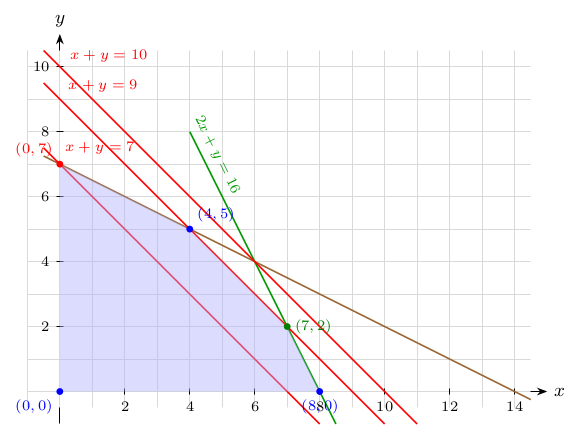
\includegraphics[width=0.85\linewidth]{figs/sensitivity-LP-tikz01.png}
\end{center}

\subsection{Ranging \( c_x \) via Reduced Costs}

To determine the range of values for \( c_x \) (the coefficient of \( x \) in the objective function) such that the current basis remains optimal, we analyze the simplex optimality conditions.

\begin{steppanel}{sensbox}
\cstep{1}{Set up the reduced costs}
The objective function is initially:
\[
    z = 2x + 3y.
\]
The cost vector for all variables is:
\[
    c = \begin{bmatrix} c_x \\ 3 \\ 0 \\ 0 \\ 0 \end{bmatrix}.
\]
The cost vector corresponding to the basic variables \( x, y, s_2 \) (i.e., the basis) is:
\[
    c_B = \begin{bmatrix} c_x & 3 & 0 \end{bmatrix}.
\]
The reduced cost for any non-basic variable \( j \) is given by:
\[
    \bar{c}_j = c_j - c_B A_B^{-1} A_j.
\]
The non-basic variables are \( s_1 \) and \( s_3 \). We need to ensure that their reduced costs remain non-positive.
\end{steppanel}

\begin{steppanel}{sensbox}
\cstep{2}{Compute the reduced costs for \( s_1 \) and \( s_3 \)}
The constraint matrix is:
\[
    A = \begin{bmatrix}
    1 & 1 & 1 & 0 & 0 \\
    2 & 1 & 0 & 1 & 0 \\
    1 & 2 & 0 & 0 & 1
    \end{bmatrix}.
\]
Extracting the columns corresponding to \( s_1 \) and \( s_3 \):
\[
    A_{s_1} = \begin{bmatrix} 1 \\ 0 \\ 0 \end{bmatrix}, \quad
    A_{s_3} = \begin{bmatrix} 0 \\ 0 \\ 1 \end{bmatrix}.
\]
Using the inverse basis matrix:
\[
    A_B^{-1} A_{s_1} =
    \begin{bmatrix}
    2 & 0 & -1 \\
    -1 & 0 & 1 \\
    -3 & 1 & 1
    \end{bmatrix}
    \begin{bmatrix} 1 \\ 0 \\ 0 \end{bmatrix} =
    \begin{bmatrix} 2 \\ -1 \\ -3 \end{bmatrix}.
\]
\[
    A_B^{-1} A_{s_3} =
    \begin{bmatrix}
    2 & 0 & -1 \\
    -1 & 0 & 1 \\
    -3 & 1 & 1
    \end{bmatrix}
    \begin{bmatrix} 0 \\ 0 \\ 1 \end{bmatrix} =
    \begin{bmatrix} -1 \\ 1 \\ 1 \end{bmatrix}.
\]
Thus, the reduced costs are:
\[
    \bar{c}_{s_1} = 0 - \begin{bmatrix} c_x & 3 & 0 \end{bmatrix} \cdot \begin{bmatrix} 2 \\ -1 \\ -3 \end{bmatrix}
    = 0 - (2c_x - 3).
\]
\[
    \bar{c}_{s_3} = 0 - \begin{bmatrix} c_x & 3 & 0 \end{bmatrix} \cdot \begin{bmatrix} -1 \\ 1 \\ 1 \end{bmatrix}
    = 0 - (-c_x + 3).
\]
\end{steppanel}

\begin{steppanel}{sensbox}
\cstep{3}{Read the range}
To retain optimality, we want $\bar{c}_{s_1}$ and $\bar{c}_{s_3}$ to be $\leq 0$:
\[
    -2c_x + 3 \leq 0 \quad \Rightarrow \quad c_x \geq \frac{3}{2} = 1.5,
\]
\[
    c_x - 3 \leq 0 \quad \Rightarrow \quad c_x \leq 3.
\]
For the current basis to remain optimal, \( c_x \) must satisfy:
\[
    \boxed{1.5 \leq c_x \leq 3},
\]
matching the range found with the dictionary in Section~\ref{sec:sensitivity-cost}.
\end{steppanel}

\begin{center}
\altincludegraphics[scale = 0.3]{Figures/sensitivity-objective}{Feasible region in the x-y plane with several level curves of the objective z = c_x x + 3y drawn for different slopes. The figure shows that as long as c_x lies in the interval [1.5, 3], the level curves tilt within the cone defined by the active constraints at the current optimum, so the optimal vertex (and basis) does not change.}
\end{center}

\section{Sensitivity Reports in Software}
\label{sec:sensitivity-software}

When solving a problem in Excel, you can ask for a sensitivity analysis.

\begin{center}
\altincludegraphics[scale =0.3]{Figures/excel-sensitivity}{Screenshot of Excel's Solver Results dialog with the option to generate a Sensitivity report selected, illustrating how to request post-optimal sensitivity output after solving a linear program.}
\end{center}
This will generate a report that will show the following:
\begin{itemize}
\item \textbf{Allowable Increase/Decrease:} For each decision variable's coefficient in the objective function, the report provides the range (allowable increase and allowable decrease) within which the coefficient can change without altering the current optimal basis. This range indicates the stability of the optimal solution with respect to changes in that coefficient.

\item \textbf{Right-Hand Side (RHS) Values:} For each constraint, the sensitivity report lists the \emph{shadow price} (or dual value), which represents the rate of change in the objective function per unit increase in the RHS of that constraint. It also provides the allowable increase and allowable decrease for the RHS. These values indicate how robust the constraints are; small allowable changes might imply that the solution is sensitive to fluctuations in available resources or demand levels.

\item \textbf{Constraint Status:} The report shows which constraints are binding (active) and which are non-binding. A binding constraint has a positive shadow price and restricts the optimal solution, while a non-binding constraint has a shadow price of zero.
\end{itemize}

These are exactly the quantities computed by hand in Sections~\ref{sec:sensitivity-rhs} and~\ref{sec:sensitivity-cost}: the allowable increase/decrease columns are the ranges from the two recipe cards, and the shadow prices are the rates from the Shadow Prices remark.

For concreteness, the figures below show a worksheet set up for Solver and the
sensitivity report it produces. Figure~\ref{fig:excel-setup} shows the model
layout --- decision-variable cells, a SUMPRODUCT objective cell, and the
constraint formulas --- and Figure~\ref{fig:excel-sensitivity-report} shows the
resulting report, with the allowable ranges, shadow prices, and binding status
described above.

\begin{figure}[h!]
\centering
\altincludegraphics[scale = 0.3]{Figures/excel-setup}{Screenshot of an Excel worksheet set up for a linear program: decision-variable cells, an objective-function cell using SUMPRODUCT, and constraint left-hand-side formulas alongside their right-hand-side values, ready for Solver.}
\caption{An Excel worksheet laid out for Solver, with decision-variable cells, a SUMPRODUCT objective, and constraint formulas.}
\label{fig:excel-setup}
\end{figure}

\begin{figure}[h!]
\centering
\altincludegraphics[scale = 0.3]{Figures/excel-sensitivity-report}{Screenshot of an Excel Solver sensitivity report. The Variable Cells table lists each decision variable's final value, reduced cost, objective coefficient, and allowable increase/decrease; the Constraints table lists each constraint's final value, shadow price, RHS, and allowable increase/decrease, identifying binding versus non-binding constraints.}
\caption{The Solver sensitivity report: variable cells (final value, reduced cost, objective coefficient, allowable increase/decrease) and constraints (final value, shadow price, RHS, allowable increase/decrease).}
\label{fig:excel-sensitivity-report}
\end{figure}

\section{Exercises}

\exgroup{Warm-ups}

\begin{ex}{Shadow Prices from the Final Dictionary}{}
\stars{1} Recall the final dictionary of the running example of this chapter:
\[
\begin{aligned}
z &= 23 - s_1 - s_3 \\
x &= 4 - 2s_1 + s_3 \\
y &= 5 + s_1 - s_3 \\
s_2 &= 3 + 3s_1 - s_3.
\end{aligned}
\]
\begin{enumerate}
\item Read off the shadow price of each of the three constraints (hours, flour, sugar) directly from the objective row.
\item Which constraint is not binding at the optimum? How can you see this in the dictionary, and how is it reflected in that constraint's shadow price?
\item The bakery is offered one extra unit of sugar for \$0.75. Should it accept? What is the most it should pay?
\end{enumerate}
\exrefs{\S\ref{sec:sensitivity-rhs}}
\end{ex}

\begin{ex}{RHS Sensitivity Range}{}
\label{ex:sensitivity-rhs-range}
\stars{1} Consider the following linear program and its optimal dictionary:
\[
\begin{aligned}
\max \quad & 4x_1 + 3x_2 \\
\st \quad
& x_1 + x_2 \leq 10 \\
& 2x_1 + x_2 \leq 16 \\
& x_1, x_2 \geq 0
\end{aligned}
\]
The optimal dictionary is:
\[
\begin{aligned}
z &= 36 - 2s_1 - s_2 \\
x_1 &= 6 + s_1 - s_2 \\
x_2 &= 4 - 2s_1 + s_2 \\
\end{aligned}
\]
with basis $B = \{x_1, x_2\}$ and nonbasic variables $N = \{s_1, s_2\}$.

Determine the range of values for $b_1$ (the RHS of the first constraint) for which the current basis remains optimal.
\exrefs{\S\ref{sec:sensitivity-rhs}}
\end{ex}

\exgroup{Core problems}

\begin{ex}{Objective Coefficient Sensitivity}{}
\stars{2} Using the same linear program and optimal dictionary as in Exercise~\ref{ex:sensitivity-rhs-range}, determine the range of values for the objective coefficient $c_1$ (the coefficient of $x_1$ in the objective function) such that the current basis remains optimal. How does the optimal objective value change as $c_1$ varies within this range?
\exrefs{\S\ref{sec:sensitivity-cost}}
\end{ex}

\begin{ex}{Full Sensitivity Workup}{}
\label{ex:sensitivity-workup-2x2}
\stars{2} A shop assembles two products with profits \$5 and \$6 per unit:
\[
\begin{aligned}
\max \quad & 5x_1 + 6x_2 \\
\st \quad
& x_1 + 2x_2 \leq 16 \quad \text{(assembly hours)} \\
& 3x_1 + 2x_2 \leq 24 \quad \text{(machine hours)} \\
& x_1, x_2 \geq 0
\end{aligned}
\]
\begin{enumerate}
\item Solve the LP (graphically or by the simplex method) and report the optimal solution and objective value.
\item Compute the shadow price of each constraint.
\item Find the allowable range of $b_1$ and of $b_2$ over which the current basis remains optimal, and state how $z$ changes inside each range.
\item Find the allowable range of $c_1$ and of $c_2$ over which the current basis remains optimal.
\item Check your answers with software (for example \texttt{scipy.optimize.linprog} or Excel Solver).
\end{enumerate}
\exrefs{\S\ref{sec:sensitivity-rhs}, \S\ref{sec:sensitivity-cost}, \S\ref{sec:sensitivity-matrix}}
\end{ex}

\begin{ex}{Ranging a Basic and a Nonbasic Coefficient}{}
\label{ex:sensitivity-obj-nonbasic}
\stars{2} Consider the LP
\[
\begin{aligned}
\max \quad & 5x_1 + 2x_2 \\
\st \quad
& 2x_1 + x_2 \leq 10 \\
& x_1 + 3x_2 \leq 15 \\
& x_1, x_2 \geq 0,
\end{aligned}
\]
whose optimal solution is $(x_1, x_2) = (5, 0)$ with $z^* = 25$ and basis $B = \{x_1, s_2\}$.
\begin{enumerate}
\item Verify that $(5,0)$ is optimal by computing the reduced costs of the nonbasic variables $x_2$ and $s_1$.
\item Find the range of the coefficient $c_2$ of the \emph{nonbasic} variable $x_2$ for which the current basis remains optimal. How does $z^*$ change as $c_2$ moves inside this range?
\item Find the range of the coefficient $c_1$ of the \emph{basic} variable $x_1$ for which the current basis remains optimal. How does $z^*$ change inside this range?
\item Explain the structural difference between the two cases: why does one range have a single finite endpoint driven by one reduced cost, while the other involves every reduced cost?
\end{enumerate}
\exrefs{\S\ref{sec:sensitivity-cost}, \S\ref{sec:sensitivity-overview}}
\end{ex}

\begin{ex}{Sensitivity from the Basis Inverse}{}
\label{ex:sensitivity-basis-inverse}
\stars{2} Consider the LP:
\[
\begin{aligned}
\max \quad & 5x_1 + 4x_2 \\
\st \quad
& x_1 + x_2 + s_1 = 6 \\
& 3x_1 + 2x_2 + s_2 = 15 \\
& x_1, x_2, s_1, s_2 \geq 0
\end{aligned}
\]
The optimal basis is $B = \{x_1, x_2\}$ with basis matrix and its inverse:
\[
A_B = \begin{bmatrix} 1 & 1 \\ 3 & 2 \end{bmatrix}, \quad
A_B^{-1} = \begin{bmatrix} -2 & 1 \\ 3 & -1 \end{bmatrix}.
\]
\begin{enumerate}
\item Compute $\mathbf{x}_B = A_B^{-1}\mathbf{b}$ and verify this gives a feasible basic solution.
\item For the RHS vector $\mathbf{b} = \begin{bmatrix} 6 \\ 15 \end{bmatrix}$, find the range of $b_1$ for which the current basis remains feasible.
\item Compute the reduced costs of the nonbasic variables. For what range of $c_1$ does the current basis remain optimal?
\end{enumerate}
\exrefs{\S\ref{sec:sensitivity-matrix}}
\end{ex}

\begin{ex}{Reading a Sensitivity Report}{}
\stars{2} The following is a sensitivity report from Excel Solver for a maximization LP with two decision variables $x_1$ and $x_2$ and three constraints:

\begin{center}
\renewcommand{\arraystretch}{1.3}
\begin{tabular}{@{}lcccc@{}}
\toprule
\textbf{Variable} & \textbf{Value} & \textbf{Obj.\ Coeff.} & \textbf{Allow.\ Increase} & \textbf{Allow.\ Decrease} \\
\midrule
$x_1$ & 8 & 6 & 2 & 3 \\
$x_2$ & 4 & 5 & 4 & 1 \\
\bottomrule
\end{tabular}
\end{center}

\begin{center}
\renewcommand{\arraystretch}{1.3}
\begin{tabular}{@{}lcccc@{}}
\toprule
\textbf{Constraint} & \textbf{Shadow Price} & \textbf{RHS} & \textbf{Allow.\ Increase} & \textbf{Allow.\ Decrease} \\
\midrule
1 & 2.5 & 20 & 4 & 6 \\
2 & 0 & 30 & $\infty$ & 5 \\
3 & 1.0 & 12 & 3 & 2 \\
\bottomrule
\end{tabular}
\end{center}

\begin{enumerate}
\item What is the current optimal objective value?
\item If the objective coefficient of $x_1$ changes from 6 to 7.5, does the optimal basis change?
\item Which constraint is non-binding? How can you tell from the report?
\item If 2 additional units of the first resource become available (RHS increases from 20 to 22), what is the new approximate optimal objective value?
\end{enumerate}
\exrefs{\S\ref{sec:sensitivity-software}}
\end{ex}

\exgroup{Concepts and connections}

\begin{ex}{Shadow Price Interpretation}{}
\label{ex:shadow-price-workshop}
\stars{2} A furniture workshop produces tables and chairs. The linear program is:
\[
\begin{aligned}
\max \quad & 50x_1 + 30x_2 \quad \text{(profit in dollars)}\\
\st \quad
& 4x_1 + 2x_2 \leq 40 \quad \text{(wood in board-feet)} \\
& 2x_1 + 3x_2 \leq 30 \quad \text{(labor in hours)} \\
& x_1, x_2 \geq 0
\end{aligned}
\]
The optimal solution is $x_1 = 7.5$, $x_2 = 5$, with optimal profit $z^* = 525$.  The dual solution is $y_1 = 11.25$, $y_2 = 2.50$.

\begin{enumerate}
\item Interpret each shadow price in terms of the resources (wood and labor).
\item If the workshop could acquire 2 additional board-feet of wood, by approximately how much would the optimal profit increase?
\item Which resource is more valuable at the margin? Explain.
\end{enumerate}
\exrefs{\S\ref{sec:sensitivity-rhs}}
\end{ex}

\begin{ex}{Why a Slack Constraint Has Price Zero}{}
\stars{2} Explain, in your own words, why a constraint that is not binding at the optimal solution must have shadow price $0$. Give two arguments:
\begin{enumerate}
\item A geometric or economic argument: what happens to the optimal solution when you add a little more of a resource you are not fully using?
\item A dictionary argument: if the slack variable of constraint $i$ is basic and positive in the final dictionary, why does perturbing $b_i$ by a small $\Delta$ leave the objective row unchanged? (The perturbation of $b_2$ in \S\ref{sec:sensitivity-rhs} is a worked instance.)
\end{enumerate}
\exrefs{\S\ref{sec:sensitivity-rhs}, \S\ref{sec:sensitivity-overview}}
\end{ex}

\begin{ex}{Why Ranges Exist at All}{}
\stars{2} Every quantity in a sensitivity report comes with an allowable range. Explain why.
\begin{enumerate}
\item What single object stays fixed throughout a sensitivity computation, and what two kinds of conditions (one for RHS changes, one for cost changes) must it continue to satisfy?
\item Why is the effect of a data change on $z^*$ \emph{linear} inside the range?
\item What happens, in terms of the simplex method, the moment a perturbation crosses an endpoint of its range?
\end{enumerate}
\exrefs{\S\ref{sec:sensitivity-overview}, \S\ref{sec:sensitivity-rhs}, \S\ref{sec:sensitivity-cost}}
\end{ex}

\begin{ex}{When the Shadow Price Prediction Breaks}{}
\stars{2} Consider the LP
\[
\max \; x_1 + x_2 \quad \st \quad x_1 \leq 1, \quad x_2 \leq 1, \quad x_1 + x_2 \leq 2, \quad x_1, x_2 \geq 0,
\]
whose optimal solution is $(1,1)$ with $z^* = 2$. Note that all three constraints are tight there, but only two of them are needed to define the vertex: the optimal solution is \emph{degenerate}.
\begin{enumerate}
\item Show that increasing $b_3$ from $2$ to $3$ does not change $z^*$, while decreasing $b_3$ from $2$ to $1$ decreases $z^*$ by $1$.
\item What, then, is ``the'' shadow price of the third constraint? Explain informally why a single number cannot describe both directions here.
\item Why should you be cautious when reading the shadow price of a degenerate LP from a solver report?
\end{enumerate}
\exrefs{\S\ref{sec:sensitivity-rhs}, \S\ref{sec:sensitivity-software}}
\end{ex}

\exgroup{Challenge problems}

\begin{ex}{Pushing Past the Range}{}
\label{ex:sensitivity-range-boundary}
\stars{3} Construct a linear program with a constraint whose shadow price is some $p > 0$ such that increasing the right-hand side of that constraint by $1$ increases the optimal value by exactly $p$, but increasing it by $5$ increases the optimal value by strictly less than $5p$. Explain what happens at the boundary of the allowable range that makes the prediction fail, and verify your construction by solving the perturbed LPs. (Hint: the running example of this chapter already contains such a constraint.)
\exrefs{\S\ref{sec:sensitivity-rhs}, \S\ref{sec:sensitivity-overview}}
\end{ex}

\subsubsection*{Selected Solutions}

\begin{solution}(Exercise~\ref{ex:sensitivity-workup-2x2})
\begin{enumerate}
\item Both constraints are binding at the optimum: solving $x_1 + 2x_2 = 16$ and $3x_1 + 2x_2 = 24$ gives $(x_1, x_2) = (4, 6)$ with $z^* = 5(4) + 6(6) = 56$.
\item The basis is $B = \{x_1, x_2\}$ with
\[
A_B = \begin{bmatrix} 1 & 2 \\ 3 & 2 \end{bmatrix}, \qquad
A_B^{-1} = \begin{bmatrix} -\tfrac12 & \tfrac12 \\[2pt] \tfrac34 & -\tfrac14 \end{bmatrix},
\]
so the shadow prices are $\mathbf{y}^\top = \mathbf{c}_B^\top A_B^{-1} = [5, 6]\,A_B^{-1} = [2, 1]$: an assembly hour is worth \$2 and a machine hour \$1.
\item With $\mathbf{b} = (b_1, 24)$, feasibility of $\mathbf{x}_B = A_B^{-1}\mathbf{b} = \left(-\tfrac{b_1}{2} + 12,\ \tfrac{3b_1}{4} - 6\right) \geq \mathbf{0}$ gives $8 \leq b_1 \leq 24$, with $z = 56 + 2(b_1 - 16)$ inside the range.  With $\mathbf{b} = (16, b_2)$, feasibility of $\left(\tfrac{b_2}{2} - 8,\ 12 - \tfrac{b_2}{4}\right) \geq \mathbf{0}$ gives $16 \leq b_2 \leq 48$, with $z = 56 + (b_2 - 24)$.
\item With $\mathbf{c}_B = (c_1, 6)$ the dual prices are $\left(-\tfrac{c_1}{2} + \tfrac92,\ \tfrac{c_1}{2} - \tfrac32\right)$; both nonnegative exactly when $3 \leq c_1 \leq 9$.  With $\mathbf{c}_B = (5, c_2)$ the dual prices are $\left(\tfrac{3c_2}{4} - \tfrac52,\ \tfrac52 - \tfrac{c_2}{4}\right)$, giving $\tfrac{10}{3} \leq c_2 \leq 10$.
\item Software confirms: at $b_1 = 8$ the solution is $(8,0)$ with $z = 40 = 56 + 2(-8)$, at $b_1 = 24$ it is $(0,12)$ with $z = 72 = 56 + 2(8)$, and just outside these values the duals change, signaling a new basis.
\end{enumerate}
\end{solution}

\begin{solution}(Exercise~\ref{ex:sensitivity-basis-inverse})
\begin{enumerate}
\item
\[
\mathbf{x}_B = A_B^{-1}\mathbf{b} = \begin{bmatrix} -2 & 1 \\ 3 & -1 \end{bmatrix}\begin{bmatrix} 6 \\ 15 \end{bmatrix} = \begin{bmatrix} 3 \\ 3 \end{bmatrix},
\]
so $(x_1, x_2) = (3, 3) \geq \mathbf{0}$ is a feasible basic solution with objective value $z = 5(3) + 4(3) = 27$.
\item Replacing $b_1$ by a variable value,
\[
\mathbf{x}_B(b_1) = A_B^{-1}\begin{bmatrix} b_1 \\ 15 \end{bmatrix} = \begin{bmatrix} -2b_1 + 15 \\ 3b_1 - 15 \end{bmatrix} \geq \mathbf{0}
\quad\Longleftrightarrow\quad 5 \leq b_1 \leq 7.5.
\]
\item The dual prices are $\mathbf{y}^\top = \mathbf{c}_B^\top A_B^{-1} = [5, 4]\, A_B^{-1} = [2, 1]$, so the reduced costs of the nonbasic slacks are $\bar{c}_{s_1} = -y_1 = -2$ and $\bar{c}_{s_2} = -y_2 = -1$; both are nonpositive, confirming optimality (equivalently, $z = 27 - 2s_1 - s_2$).  With $c_1$ variable, $\mathbf{y}(c_1)^\top = [c_1, 4]\, A_B^{-1} = [-2c_1 + 12,\ c_1 - 4]$, and the basis stays optimal while both components are nonnegative:
\[
-2c_1 + 12 \geq 0 \ \text{ and } \ c_1 - 4 \geq 0
\quad\Longleftrightarrow\quad 4 \leq c_1 \leq 6.
\]
\end{enumerate}
\end{solution}

\begin{solution}(Exercise~\ref{ex:shadow-price-workshop})
At the optimal solution $(x_1, x_2) = (7.5, 5)$ both constraints are binding: $4(7.5) + 2(5) = 40$ and $2(7.5) + 3(5) = 30$.

\begin{enumerate}
\item The shadow price of wood is $y_1 = 11.25$: one additional board-foot of wood increases the optimal profit by \$11.25 (as long as the basis does not change).  The shadow price of labor is $y_2 = 2.50$: one additional hour of labor is worth \$2.50 at the margin.
\item Two additional board-feet increase profit by approximately $2 \times 11.25 = \$22.50$, from \$525 to \$547.50.  (This is exact here: the wood RHS can range from $20$ to $60$ before the basis changes, and $42$ is well inside that range.)
\item Wood is more valuable at the margin, since $11.25 > 2.50$: a unit of wood buys more additional profit than a unit of labor.
\end{enumerate}
\end{solution}

\begin{solution}(Exercise~\ref{ex:sensitivity-range-boundary})
The running example of this chapter works.  Its hours constraint $x + y \leq 9$ has shadow price $p = 1$, valid for $7 \leq b_1 \leq 10$ (allowable increase $1$).  Increasing $b_1$ by $1$ to $10$ raises the optimal value from $23$ to $24$, exactly $p$.  Increasing $b_1$ by $5$ to $14$ raises it only to $24$, not to $23 + 5 = 28$: solving the LP with $b_1 = 14$ gives the optimum $(x, y) = (6, 4)$ determined by the flour and sugar constraints, and $z^* = 2(6) + 3(4) = 24$.  At the range boundary $b_1 = 10$ the basic variable $s_2$ hits $0$ and the basis changes; beyond it the hours constraint is no longer binding, so its shadow price drops to $0$ and further increases in $b_1$ buy nothing.  In general, the optimal value is a piecewise-linear concave function of $b_1$, and the shadow price is only its slope on the current piece.
\end{solution}
